\section{3D coordination algorithms}

\begin{frame}
	\frametitle{Motivation}
	\centering
	\href{mbzirc_video.mp4}{\includegraphics[width=0.8\textwidth]{figures/mbzirc_screen.jpg}}
	
\end{frame}

\subsection{Extension of 2D exploration solutions to 3D solution}
\begin{frame}
     \frametitle{Extension of 2D exploration solutions to 3D}
     \begin{itemize}
     	\item[-] Reducing the dimension of the navigation space of robots\footcite{Bachrach2009}$\,$\footcite{Surmann2003}
     	\begin{itemize}
     		\item[-] 2.5D elevation maps 
     		%\item[-] Resulting model would probably contain unexplored areas
     	\end{itemize}	
     	\item[-] A complete 3D exploration is proposed in 2013 by Dornhege\footcite{Dornhege2013}
%     	algorithm was tested on a 5-DOF manipulator with a workspace radius of one
%     	meter
     	 %(i.e., an extension of Next-Best-View method to 3D)
     	 	\begin{itemize}
     			\item[-] Can be applied only in small areas (\textbf{computational effort})
     	 	\end{itemize}
      	\item[-] Combination of 2D and 3D exploration strategies\footcite{Maurovic2014}
      	%based on next-best-view method and room detection (Maurovic\footcite{Maurovic2014})
      	\begin{itemize}
      		\item[-] The robot switches to 3D exploration while a room is detected
      		\item[-] Local maps of rooms
      		% are used to overcome the problem of computational effort and memory consumption
      	\end{itemize}		
     \end{itemize}   
\end{frame}

\subsection{3D exploration - single robot}
\begin{frame}
	\frametitle{3D exploration - single robot}
	\begin{itemize}
		\item[-] Formalized extension of the \textbf{frontier-based exploration}\footcite{ShadeNewman2011}
		\item[-] Next-best-view approach for 3D exploration\footcite{Bircher2016}
		
%		Shade and Newmann formalize, in [15], the 3D extension of
		%the frontier-based exploration. In particular, 3D frontiers are integrated with a
		%vector field approach to achieve 3D exploration with a stereo camera. 
		%3D requires highmemory and computational consumptions
		\item[-] Extraction of 3D frontiers from the OctoMap\footcite{Zhu2015}
%		\begin{itemize}
%			\item[-] Extract the 3D	frontiers from the OctoMap
%		\end{itemize}
		\item[-] 3D exploration based on surface frontier voxels \footcite{Senarathne2016} 
		\begin{figure}
			\centering
			\includegraphics[width=0.5\textwidth]{figures/senarathne}
		\end{figure}
		
%presented an alternative approach to 3D exploration based on surface frontier voxels. The strategy focuses on seeking the expansion of mapped surfaces, instead of reducing unmapped voxels.
		
	\end{itemize}	
\end{frame}
%Next-best-view approach in the process of building 3D model of a real object used without any a priori information about the environment was described in \cite{VasquezGomez2014}. The algorithm determines each view to reconstruct an arbitrary object. Furthermore, authors proposed a method to deal with the uncertainty in sensor positioning.
%Next-best-view approach for 3D exploration was presented by Bircher et. al. \cite{Bircher2016}. Authors presented a novel path planning algorithm for the autonomous exploration of an unknown area. The proposed planner finds the best branch in an online computed tree. The quality of the branch is determined by the amount of unmapped space that can be explored. The planner is capable of running online, onboard a robot with limited resources.
%\begin{frame}
%     \frametitle{Extension of 2D exploration solutions to 3D (3)}
%		\begin{itemize}
%			\item[-]  for indoor environment
%			\item[-] Frontiers are searched just on a subset of nodes, the changed cells\footcite{Keidar2012}
%			\item[-] Method suffers from local minima
%			\item[-] The application in uncluttered environments results in few uninformative frontiers
%		\end{itemize}
%\end{frame}
\subsection{3D exploration - multi-robot}
\begin{frame}
	\frametitle{3D exploration - multi-robot}
	\begin{itemize}
		\item[-] An entropy-based measure of information utility\footcite{Rocha2005}
		% to define a cooperation strategy for sharing useful information
		\item[-] Minimization of accumulative data errors during the exploration\footcite{Vutetakis2019}
		\item[-] An information potential field based method\footcite{Wang2019} 
		\begin{itemize}
			\item[-] Reduce path cost and map entropy (an uncertainty of the map)
		\end{itemize} 
		\begin{figure}
			\centering
			\includegraphics[height=2cm]{figures/frontier_extraction}
		\end{figure}
%Vutetakis in \cite{Vutetakis2019} proposed a novel strategy for inspecting critical infrastructure autonomously using Micro Aerial Vehicles (MAVs). In order to facilitate autonomous inspection capabilities, this strategy addresses the problem of autonomous MAVs exploration and coverage of an unknown structure to acquire the spatial information necessary for the development of a high-fidelity 3D model of the structure. Key to this problem is to not only cover the entire structure, but also to minimize accumulative data errors during the exploration through direct planning of loop closures. 

%Rocha et al. \cite{Rocha2005} dealt with 3D mapping by multiple robots using cubic cells for information storage. Authors presented a technique which is used for frontier-based exploration. At the beginning of the exploration an initial map is given to the robot, the robots update old map by new set of information obtained through sensing and share their useful information with other robots. The process is repeated until the whole area is explored and mapped.

%The 3D exploration problem using aerial vehicles within limited flight endurance was addressed by Wang et al. \cite{Wang2019}. Authors proposed an information potential field based method considering both the traveled cost and information-gain. The next-best-view point is chosen based on a multi-objective function which considers information of several candidate regions and the traveled path cost. The selected goal
%attracts the robot while known obstacles form the repulsive
%force repel the robot.
				
	\end{itemize}	
\end{frame}

\subsection{Firefighting mission}
\begin{frame}
	\frametitle{Firefighting mission - frontier exploration (1)}
	\begin{columns}
		\begin{column}{0.5\textwidth}\centering
			\begin{center}
				\includegraphics[height=3cm]{figures/3D_strategy}
				\label{fig:forest_uav}
			\end{center}
			%			\vspace{0.1cm}
			%			\begin{itemize}
			%				\item Stiff position-controlled
			%				\item Payload: 10-300 kg
			%				\item High speed, high accuracy
			%			\end{itemize}
		\end{column}
		\begin{column}{0.4\textwidth}\centering
		\begin{itemize}
			\item[-] GPS building location
			\item[-] Google Cartographer SLAM
		\end{itemize}
			%			\vspace{0.1cm}
			%			\begin{itemize}
			%				\item Joint torque-controlled
			%				\item Payload: up to 15 kg
			%				\item Environment sensing
			%			\end{itemize}
		\end{column}
	\end{columns}
\end{frame}

\begin{frame}
	\frametitle{Firefighting mission - frontier exploration (2)}
	\begin{figure}
		\includegraphics[height=3cm]{figures/building}
	\end{figure}
	\begin{figure}
	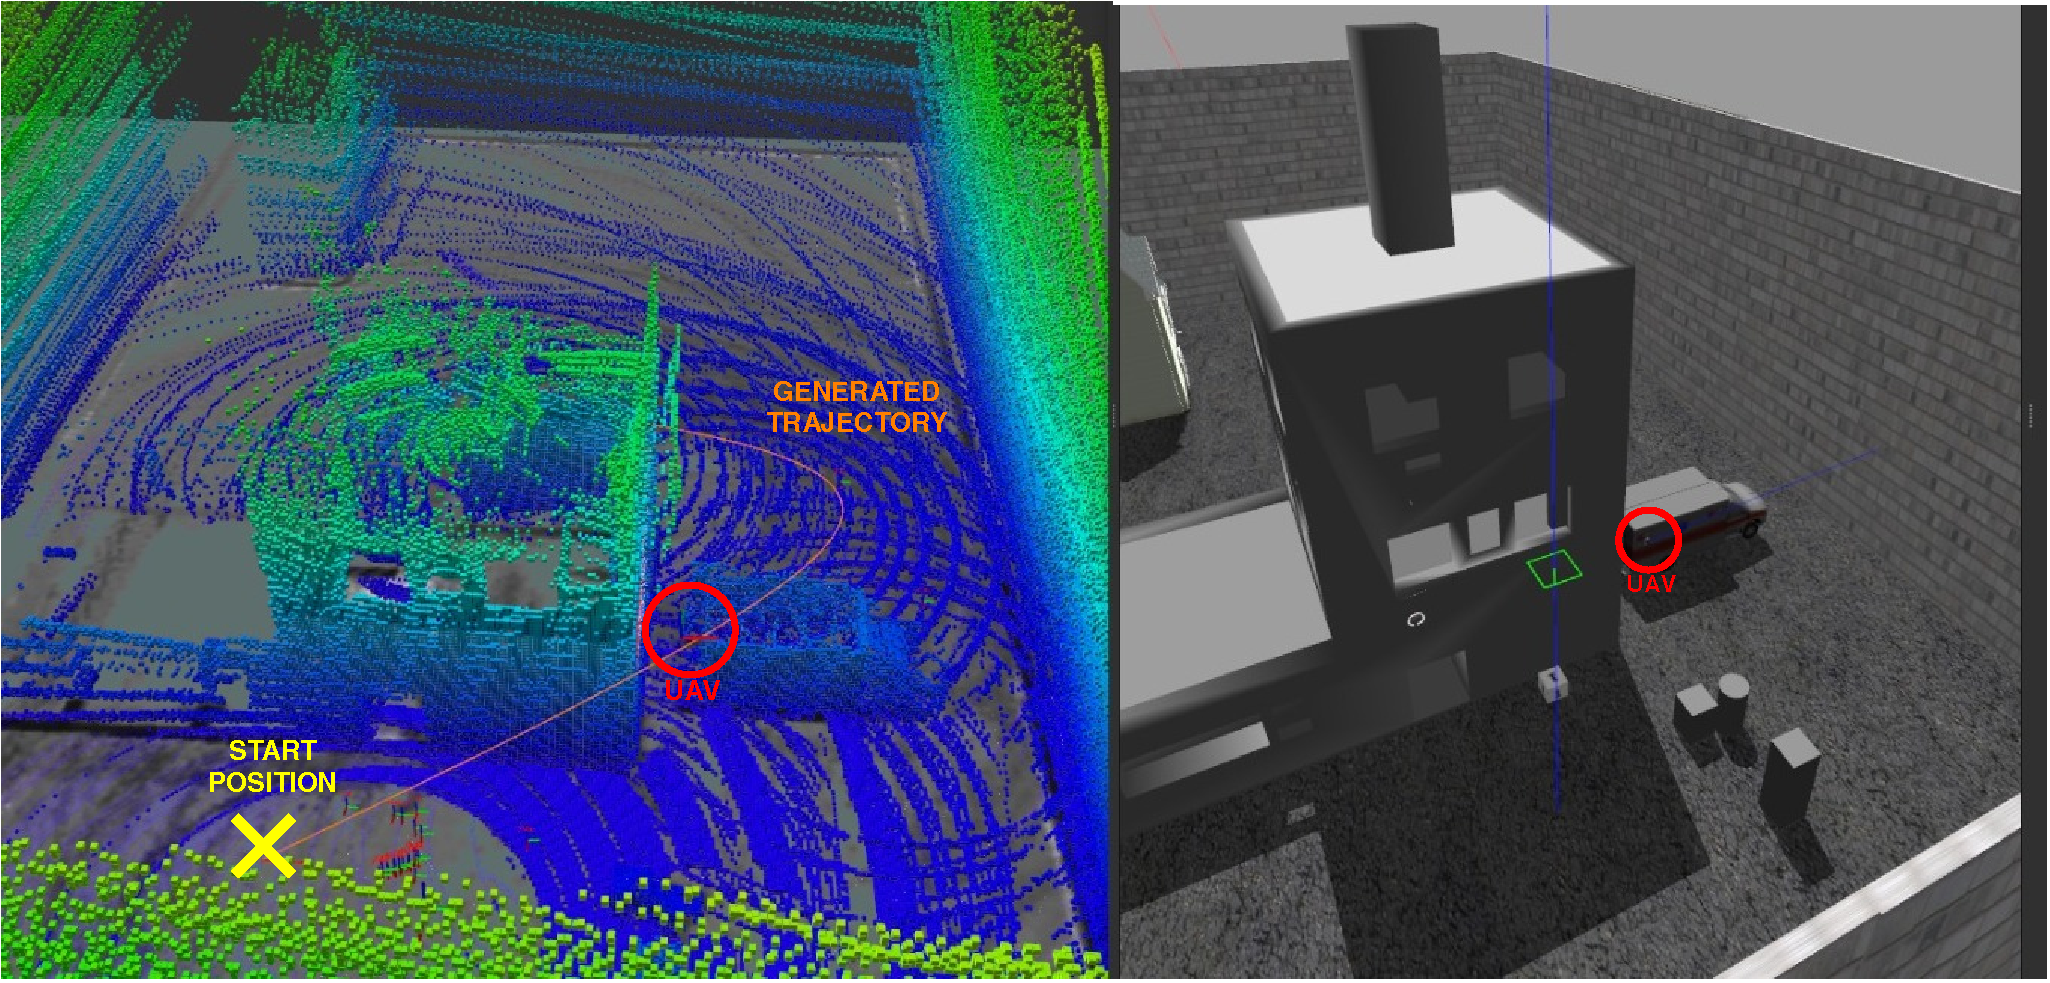
\includegraphics[height=3cm]{figures/rviz_gazebo}
	\end{figure}
		
\end{frame}

\begin{frame}
	\frametitle{Firefighting mission - real life scenario\footcite{mbzirc}}
	\begin{columns}
		\begin{column}{0.5\textwidth}\centering
			\begin{center}
				\includegraphics[width=1\textwidth]{figures/mbzirc_1}
				\label{fig:forest_uav}
			\end{center}
		\end{column}
		\begin{column}{0.5\textwidth}\centering
			\begin{center}
				\includegraphics[width=1\textwidth]{figures/mbzirc_2}
				\label{fig:forest_uav}
			\end{center}
		\end{column}
	\end{columns}
	
\end{frame}